\documentclass[aspectratio=169,10pt]{beamer}
\usetheme{metropolis}
\usepackage{tikz}
\usepackage{booktabs}
\usepackage{graphicx}
\usetikzlibrary{arrows.meta,positioning,calc}
\graphicspath{{../../experiments/figures/}}

\title{Milestone 3}
\subtitle{Distributed Robot Control under Random Communication Delay}
\author{Cyber Physical Robotics}
\date{}

\begin{document}
\maketitle

\begin{frame}{Problem}
Every message reaches each receiver after its own random delay (exponential).
\medskip
\begin{itemize}
\item \textbf{M2 assumption:} everybody reads the same messages in the same step.
\item \textbf{Failure 1, two helpers for one goal:} each helper sees different \texttt{POS} replies and believes it is the closest.
\item \textbf{Failure 2, picks at different times:} the two \texttt{READY} messages arrive at different steps, so one robot picks alone (``only one robot picked'').
\end{itemize}
\end{frame}

\begin{frame}{Idea: separate \emph{who} from \emph{when}}
\begin{columns}[T]
\begin{column}{.48\textwidth}
\textbf{Who is the partner}\\[2pt]
Consensus with \textbf{Paxos}. Correct for any message delay.
\end{column}
\begin{column}{.48\textwidth}
\textbf{When to pick}\\[2pt]
Decided by \textbf{sensing} only. Sensing has no delay: two robots on one cell sense each other in the same step.
\end{column}
\end{columns}
\end{frame}

\begin{frame}{Messages}
\small
\begin{tabular}{@{}ll@{}}
\toprule
\texttt{FOUND} & instance, goal id, position (finder)\\
\texttt{PREPARE} & instance, ballot (Paxos 1a)\\
\texttt{PROMISE} & instance, ballot, last accepted ballot and value (1b)\\
\texttt{ACCEPT} & instance, ballot, partner id (2a)\\
\texttt{ACCEPTED} & instance, ballot, value (2b, to all learners)\\
\texttt{PICKED} & goal id, so late messages are ignored\\
\bottomrule
\end{tabular}
\medskip
\begin{itemize}
\item Instance = (goal id, finder's Lamport clock). Ballot = (Lamport clock, robot id): never equal.
\item Every robot is acceptor and learner; volunteers also propose.
\end{itemize}
\end{frame}

\begin{frame}{State machine}
\centering
\resizebox{\linewidth}{!}{%
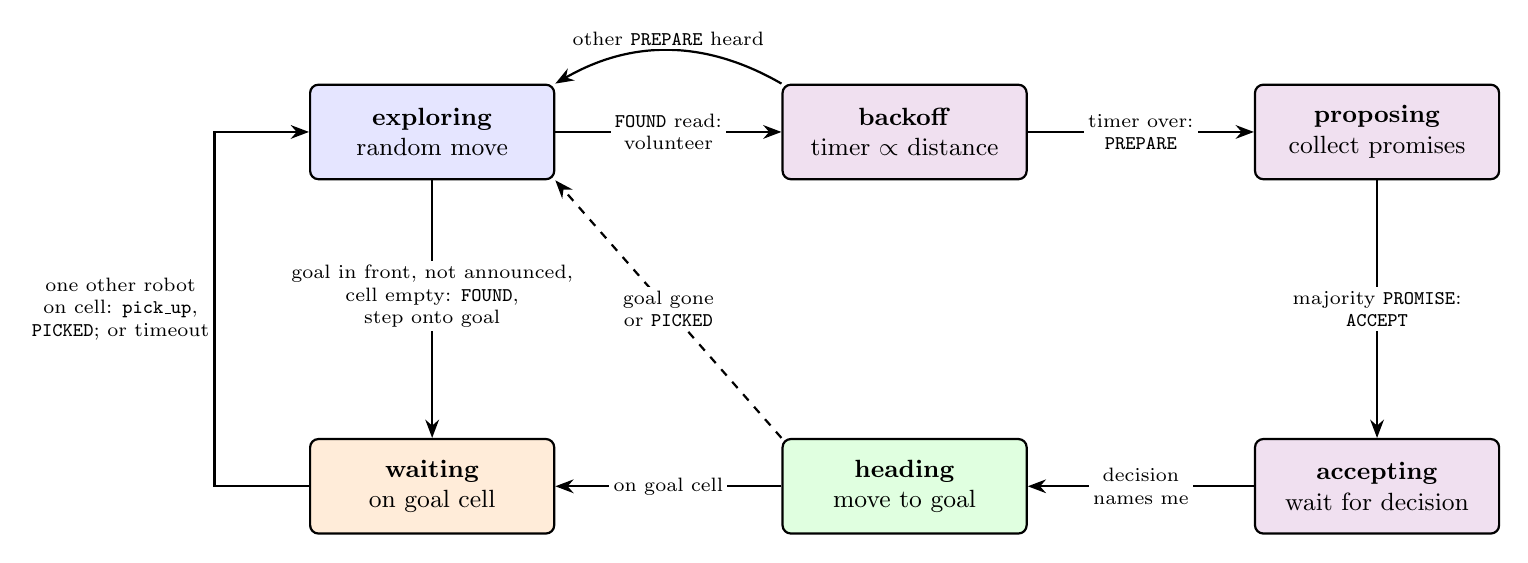
\begin{tikzpicture}[
    >=Stealth, thick,
    state/.style={draw, rounded corners=3pt, minimum width=3.1cm,
                  minimum height=1.2cm, align=center, font=\small},
    lbl/.style={font=\scriptsize, align=center, fill=white, inner sep=1.5pt}
]
\node[state, fill=blue!10]   (explore) at (0,0)     {\textbf{exploring}\\random move};
\node[state, fill=orange!15] (wait)    at (0,-4.5)  {\textbf{waiting}\\on goal cell};
\node[state, fill=violet!12] (back)    at (6,0)     {\textbf{backoff}\\timer $\propto$ distance};
\node[state, fill=violet!12] (prop)    at (12,0)    {\textbf{proposing}\\collect promises};
\node[state, fill=violet!12] (acc)     at (12,-4.5) {\textbf{accepting}\\wait for decision};
\node[state, fill=green!12]  (head)    at (6,-4.5)  {\textbf{heading}\\move to goal};

\draw[->] (explore.south) -- node[lbl, pos=.45]{goal in front, not announced,\\cell empty: \texttt{FOUND},\\step onto goal} (wait.north);
\draw[->] (explore.east) -- node[lbl, pos=.5]{\texttt{FOUND} read:\\volunteer} (back.west);
\draw[->] (back.north west) to[out=150, in=30] node[lbl, above]{other \texttt{PREPARE} heard} (explore.north east);
\draw[->] (back.east) -- node[lbl, pos=.5]{timer over:\\\texttt{PREPARE}} (prop.west);
\draw[->] (prop.south) -- node[lbl, pos=.5]{majority \texttt{PROMISE}:\\\texttt{ACCEPT}} (acc.north);
\draw[->] (acc.west) -- node[lbl, pos=.5]{decision\\names me} (head.east);
\draw[->] (head.west) -- node[lbl, pos=.5]{on goal cell} (wait.east);
\draw[->, dashed] (head.north west) -- node[lbl, pos=.5]{goal gone\\or \texttt{PICKED}} (explore.south east);
\draw[->] (wait.west) -- ++(-1.2,0) |- node[lbl, pos=.25, left]{one other robot\\on cell: \texttt{pick\_up},\\\texttt{PICKED}; or timeout} (explore.west);
\end{tikzpicture}}
\end{frame}

\begin{frame}{Paxos: why only one partner is chosen}
\begin{itemize}
\item Acceptor promises only a ballot higher than any promised; accepts only if no higher promise.
\item Learner: value chosen when a majority reports \texttt{ACCEPTED} for one ballot.
\item Any two majorities share a robot. A later proposer hears the accepted value in a promise and must re-propose it.
\item No timing assumption, so it holds for \textbf{any delay}.
\end{itemize}
\medskip
\textbf{Seen in simulator:}
\begin{itemize}
\item \emph{Late rival:} robot 4 proposed with ballot (59,4) but was forced to send value 7 (accepted at (2,7)).
\item \emph{Duelling proposers:} ballots (71,1) and (71,8): id breaks tie, all learned partner 8.
\end{itemize}
\end{frame}

\begin{frame}{Why picks are legal}
A robot picks only on its goal cell with \textbf{exactly one other robot} sensed there. Both pick in the same step.
\medskip

Entry control makes ``the other robot'' mean ``my partner'':
\begin{itemize}
\item finder steps on a goal only if the cell is empty;
\item exploring robots never step on a goal cell;
\item partner enters only if the goal is still there and at most one robot is on it;
\item picked goals are remembered; late messages ignored.
\end{itemize}
\end{frame}

\begin{frame}{Results: M2 vs M3}
\small Setup: 10$\times$10 grid, 8 robots, 20 seeds $\times$ 2000 steps per cell.
\centering
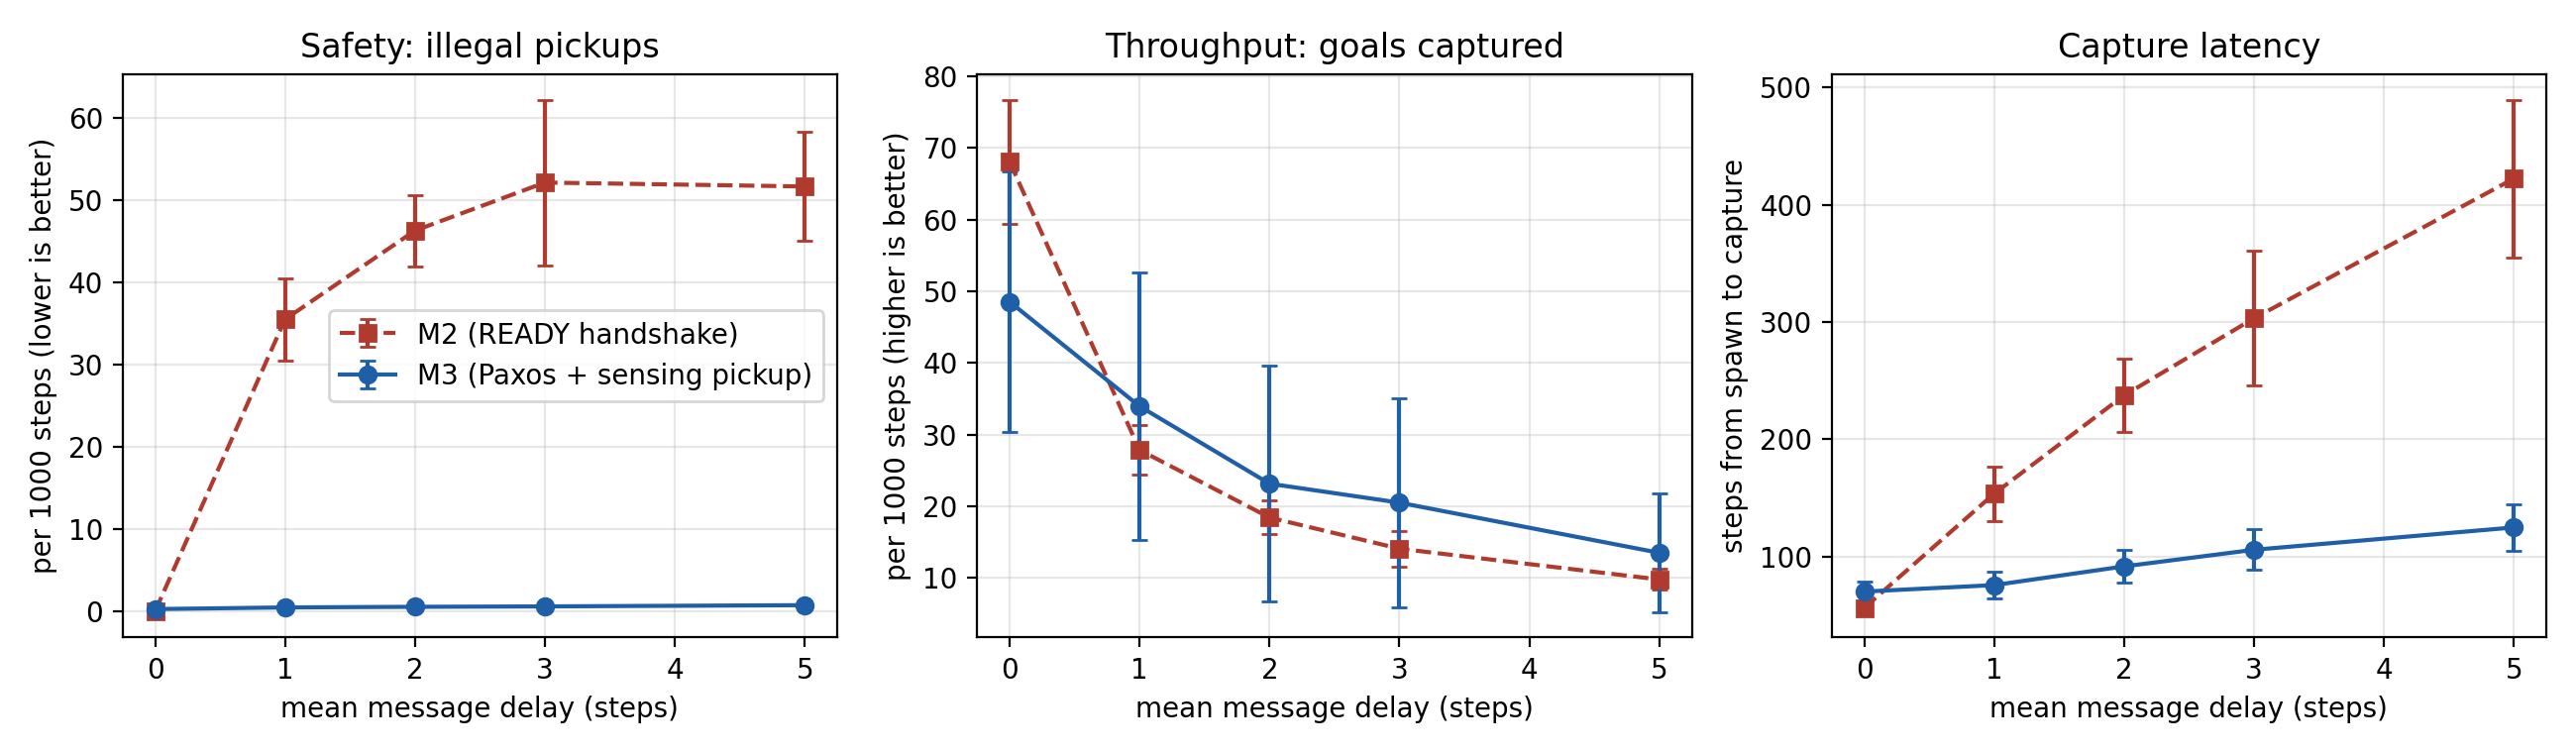
\includegraphics[width=.88\linewidth,height=.62\textheight,keepaspectratio]{m2_vs_m3.png}
\end{frame}

\begin{frame}{Results: numbers}
\centering\small
\begin{tabular}{@{}r rr rr rr@{}}
\toprule
& \multicolumn{2}{c}{Illegal / 1000 steps} & \multicolumn{2}{c}{Captures / 1000} & \multicolumn{2}{c}{Latency (steps)}\\
\cmidrule(lr){2-3}\cmidrule(lr){4-5}\cmidrule(l){6-7}
Mean delay & M2 & M3 & M2 & M3 & M2 & M3\\
\midrule
0 & 0.00 & 0.25 & 68.0 & 48.5 & 56 & 70\\
1 & 35.52 & 0.45 & 27.9 & 34.0 & 154 & 76\\
2 & 46.33 & 0.53 & 18.4 & 23.1 & 237 & 92\\
3 & 52.17 & 0.57 & 14.1 & 20.5 & 303 & 106\\
5 & 51.70 & 0.72 & 9.8 & 13.5 & 422 & 125\\
\bottomrule
\end{tabular}
\medskip
\begin{itemize}\small
\item Illegal picks cut by about \textbf{99\%} under delay. No run with two partners for one instance.
\item Delay 0: M2 faster (M3 pays backoff + two Paxos round trips).
\item Delay $\geq$1: M3 captures more; latency 70 to 125 vs 56 to 422.
\end{itemize}
\end{frame}

\begin{frame}{Scalability: 4 to 128 robots}
\centering
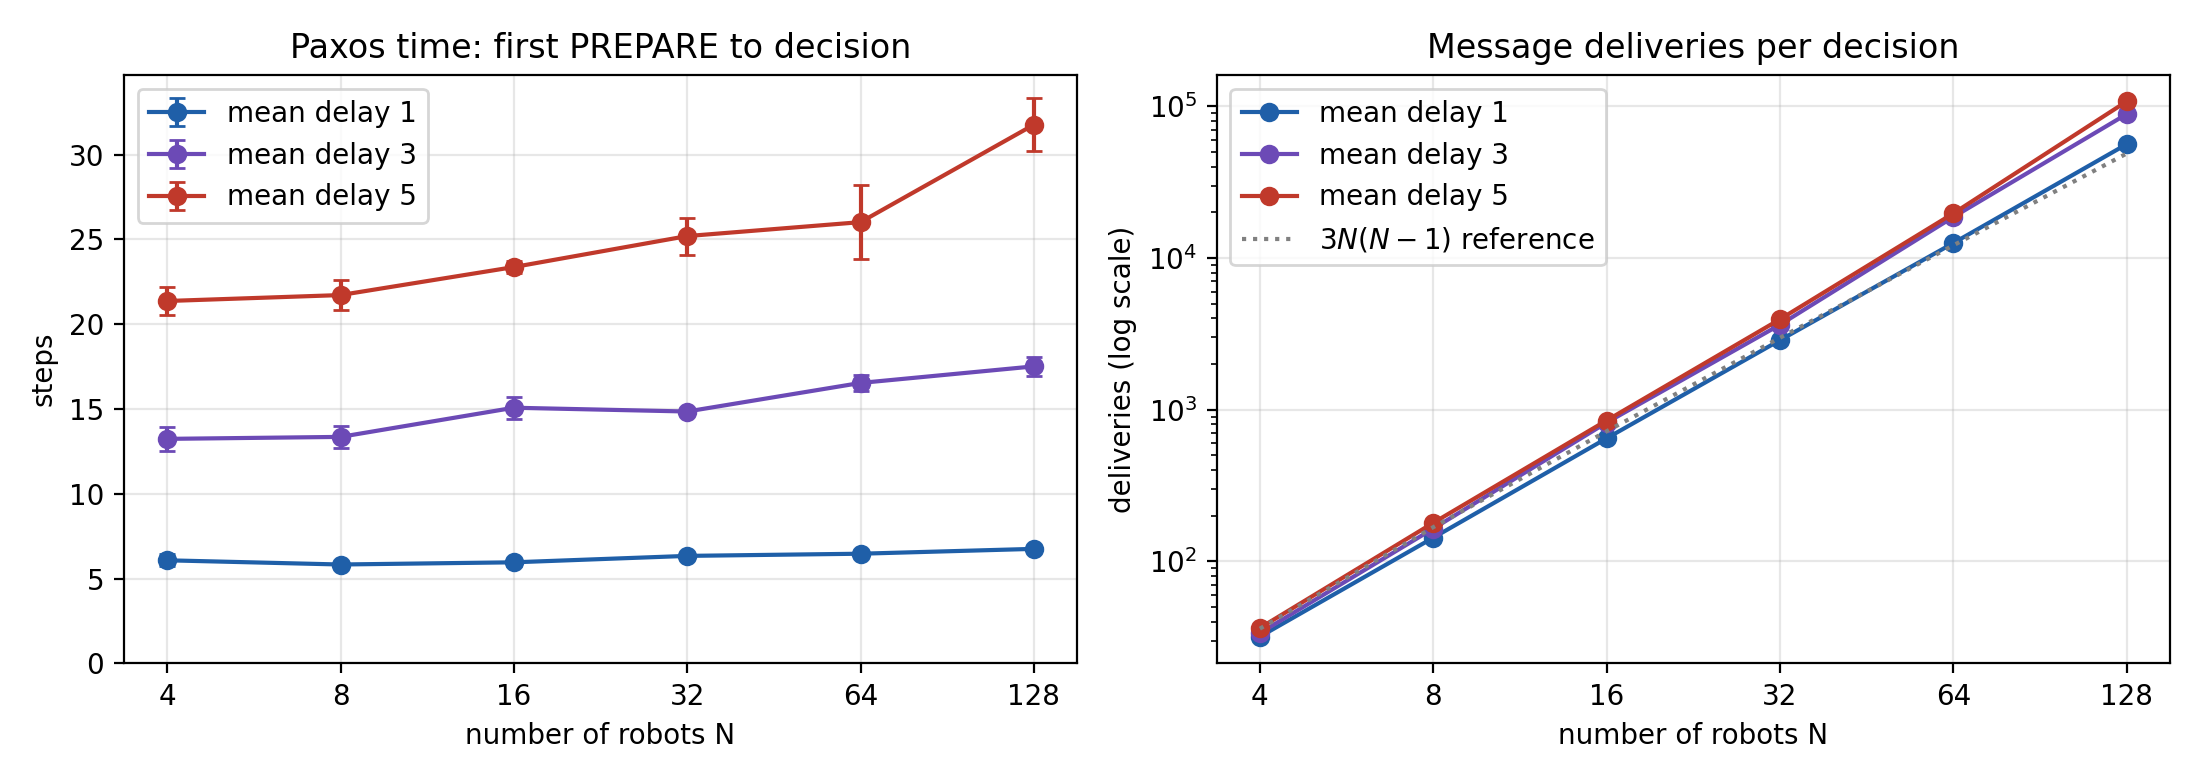
\includegraphics[width=.8\linewidth,height=.5\textheight,keepaspectratio]{scaling.png}
\begin{itemize}\small
\item \textbf{Time grows slowly:} proposer waits for the fastest majority. Delay 1: 6.1 to 6.8 steps; delay 5: 21.4 to 31.8.
\item \textbf{Messages grow as $N^2$:} about $2N(N-1)$ deliveries per decision; 32 at 4 robots, about 56\,000 at 128.
\item Fix (not implemented): small fixed acceptor group, or one Paxos group per region.
\end{itemize}
\end{frame}

\begin{frame}{Limitations}
\begin{itemize}
\item \textbf{Path crossing:} heading robot walks over another goal where a finder waits, finder picks alone. Cause of 99 of 101 illegal picks. Fix: never step on a foreign goal cell.
\item \textbf{Fixed timeouts:} 60-step wait does not adapt to delay; costs throughput, not safety.
\item \textbf{Known, fixed $N$:} majority needs $N$.
\item \textbf{No loss or crashes:} Paxos tolerates them, but a stalled proposer needs a retry timeout.
\end{itemize}
\end{frame}

\begin{frame}{Summary}
\begin{itemize}
\item Paxos decides \emph{who}; sensing decides \emph{when}.
\item Illegal picks down about 99\% under random delay; faster than M2 once delay $\geq$1.
\item Decision time scales well; message cost is the price at large $N$.
\item Next: block foreign goal cells on the path.
\end{itemize}
\centering\Large Questions?
\end{frame}

\end{document}
